
\documentclass[a4paper]{article}

\usepackage{url}
\usepackage{amsmath}
\usepackage{verbatim}   		% Useful for program listings
\usepackage[T1]{fontenc}       	% For Swedish characters ÅÄÖ etc.
\usepackage[utf8]{inputenc}
% \usepackage[swedish]{babel} % For Swedish hyphenation
\usepackage{fancyvrb}           	% For lists with tabulators
\fvset{tabsize=4}              	 	% Tabulator size
\fvset{fontsize=\small}         	% List font size
\usepackage{graphicx}		% Imports the graphicx package, useful for images

% generate clickable references & toc
\usepackage[]{hyperref}
\hypersetup{
%    pdftitle={Your title here},
%    pdfauthor={Your name here},
%    pdfsubject={Your subject here},
%    pdfkeywords={keyword1, keyword2},
    bookmarksnumbered=true,
    bookmarksopen=true,
    bookmarksopenlevel=1,
    colorlinks=true,
    pdfstartview=Fit,
    pdfpagemode=UseOutlines,    % this is the option you were lookin for
    pdfpagelayout=TwoPageRight
}

% define namedlabel as per http://texblog.org/2012/03/21/cross-referencing-list-items/
% this is used for naming the requirements.
\usepackage{enumitem, hyperref}
\usepackage{nameref}

% suggestion from http://tex.stackexchange.com/questions/1230/reference-name-of-description-list-item-in-latex
\makeatletter
\newcommand{\labitem}[2]{%
\def\@itemlabel{\textbf{#2}}
\item
\def\@currentlabel{#2}\label{#1}}
\makeatother

% just a work-in-progress idea

% usage: \usecase{cross-reference}{display-reference} text text ...
\newcommand{\usecase}[2]{
  \subsection*{#2}
  \label{#1}
  \addcontentsline{toc}{subsection}{\nameref{#1}}
}


% usage: \scenario{cross-reference}{display-reference} text text ...
\newcommand{\scenario}[2]{
  \subsubsection*{#2}
  \label{#1}
  \addcontentsline{toc}{subsubsection}{\nameref{#1}}
}

% usage: \requirement{cross-reference}{display-reference} text text ...
\newcommand{\requirement}[2]{
  \paragraph*{#2:}
  \label{#1}
  \addcontentsline{toc}{paragraph}{\nameref{#1}}
}




\title{Dragonfly Quadrotor UAV \\ System Requirements Specification}
\author{Eduardo Riffo \\ Abed Shoka}

\date{\today}
%\date{December, 2015}         		% Today's date if not specified


\begin{document}                	% Start of document

\maketitle                      	% Prints the title defined above with \title, \author and \date

\begin{center}
\vspace{64pt}

\includegraphics[scale=1.6]{images/AF_Logotype20141_Black.png}
\vspace{16pt}
\\ \large ÅF Technology
\end{center}

\vspace{16pt}
\begin{tabular}{ l l l p{8.5cm} }
	Ver. & Date & Name & Description and Reason for change \\\hline
	0.1 Draft & December 14, 2015 & Eduardo & Created document structure.\\
\end{tabular}

\begin{table}[]
\centering
\caption{Document approval}
\begin{tabular}{c c c c}
\hline\hline
Signature & Name & Title & Date \\ [0.5ex]
\hline
	& & & \\
	& & & \\
	& & & \\
\hline
\end{tabular}
\label{table:nonline}	
\end{table}

\newpage

\tableofcontents				% Insert table of contents

\newpage

\section{Introduction}

The System Requirement Specification (SRS) document is a technical description of the functional and non-functional requirements needed for the DragonFly project. A system design picture contatinening the Dragonfly system and all its subsystem is described below. This document should contain all of the information needed by a software engineer to adequately design and implement the software product described by the requirements listed in this document. 

\begin{figure}[!h]
	\centering
	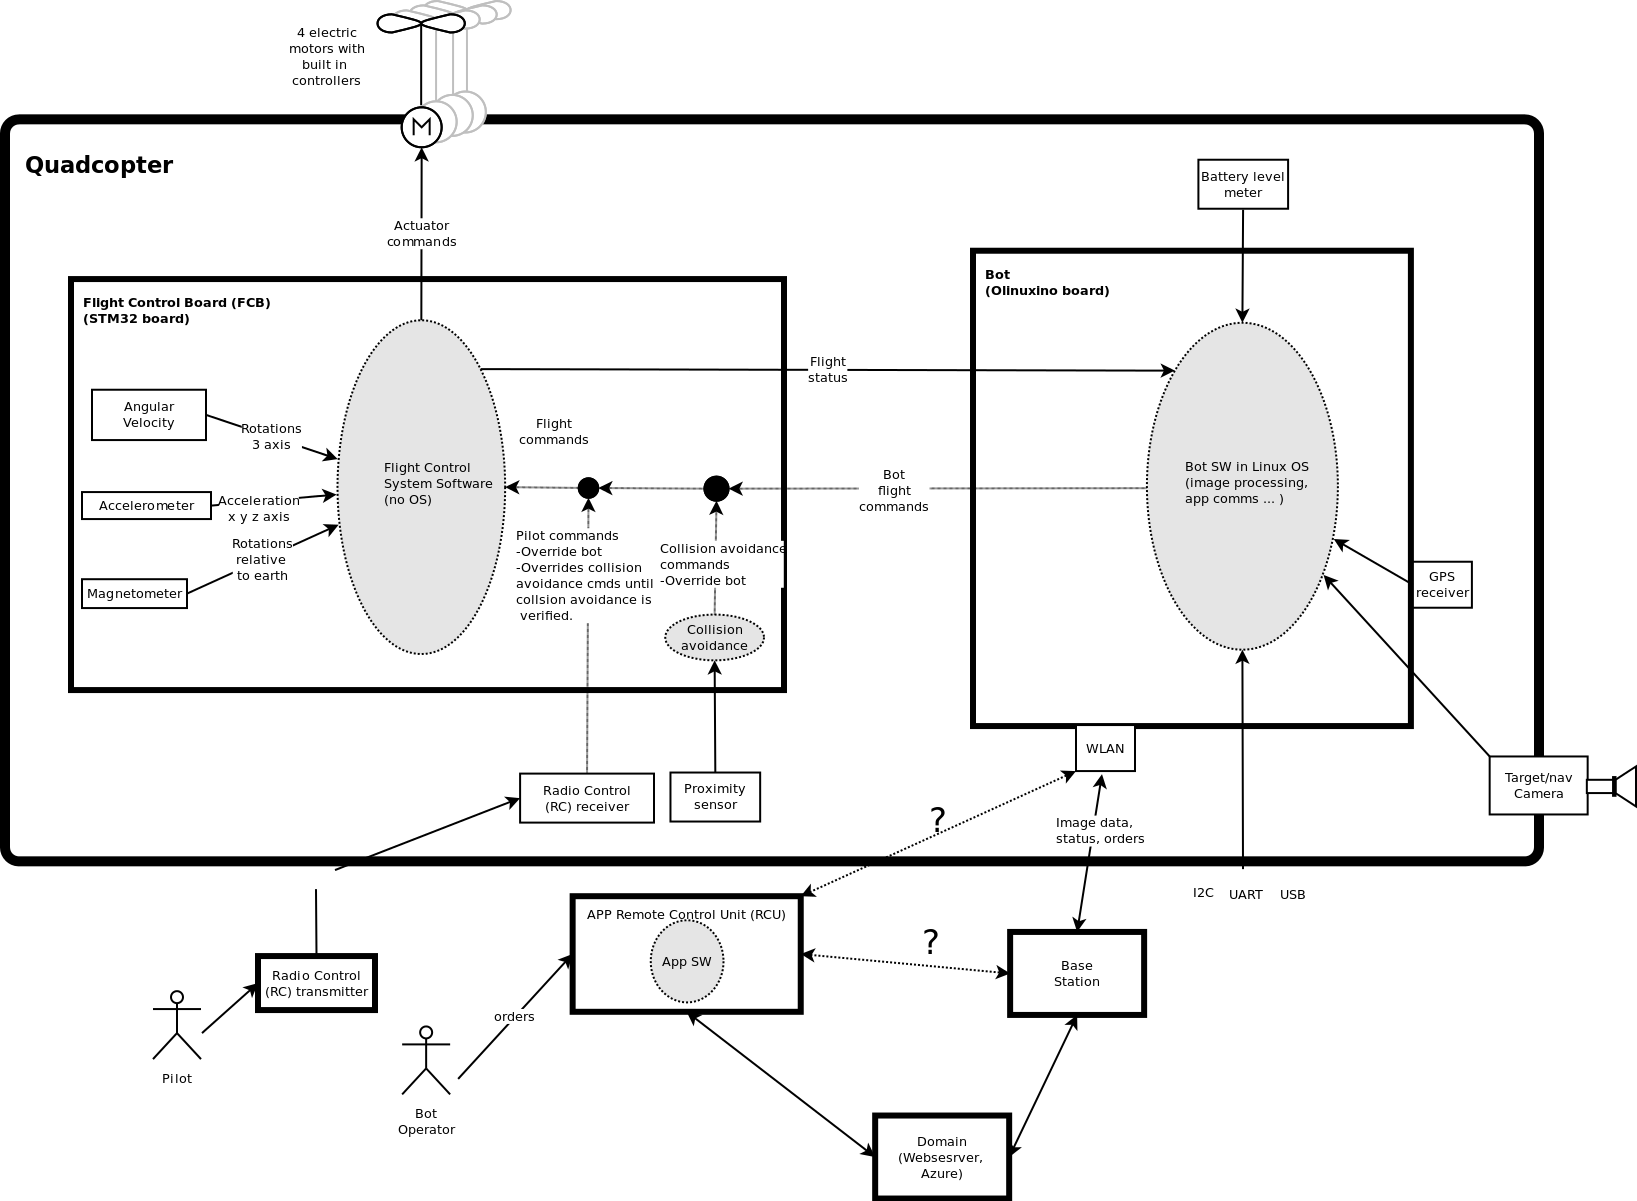
\includegraphics[width=\textwidth]{images/SystemArchitectureDiagram_DF.png}
	\caption{SystemArchitectureDiagram}
	\label{fig:sysarchdiag}
\end{figure}

\subsection{Purpose}

The purpose of this SRS in to list all the system requirements and how they map to PRS requirements and use cases. The intended audience is of this document are all involved in the dragonfly project.

\subsection{Scope}

The subsystems that are part of the dragonfly system is:
\begin{itemize}
	\item Charger subsystem. Which is responsible for controlling charge level and
	charging the Dragonfly UAV Quadcopter. It will also suggest or redirect to an available charging base. By doing so it enables optimized usage of the dragonfly from a charging point of view.
	\item subsystem X.
	\item Subsystem Y.
\end{itemize}

\subsection{Definition, Acronyms and Abbreviations}

The SRS contains the following definitions of terms, acronyms, and abbreviations required to properly interpret the SRS.
\begin{itemize}
	\item SRS - System Requirement Specification.
	\item PRS - Product Requirement Specification. 
	\item UC  - Use case definition.
	\item SoC - State of compliance.
	\item SoV - State of verification.
	\item SoI - State of implementation.
\end{itemize}

\subsection{References}

\begin{thebibliography}{99}
	\bibitem{Dragonfly-PRS} Dragonfly Product Requirement Specification, 2015
	\bibitem{Dragonfly-UC} Dragonfly Use Case Description, 2015
\end{thebibliography}

\subsection{Overview}

\section{General Description}

The SRS describes the general factors that affect the dragonfly project and its requirements on the different subsystem. It should be made clear that this section does not state specific requirements; it only makes those requirements easier to understand.

\subsection{Product Perspective}

This subsection of the SRS puts the dragonfly product into perspective with other related products requirements or projects goals. 

\subsection{Product Functions}

The summary of the product requirements are listed in \cite{Dragonfly-PRS}. 


\subsection{General Constraints}

This SRS only describes the the dragonfly and charger base as product entity, all other components that are a consired a part of the either the dragonfly or the charger base.
From a software point of view all sub-system are considered to be a part  dragonfly system.

\subsection{Assumptions and Dependencies}

This part of the SRS list each of the factors that affect the requirements stated in the SRS. These factors are not design constraints on the software but are, rather, any changes to them that can affect the requirements in the SRS. 
It is assumed that the fligth control board (FCB) runs a freeRTOS and has an interface to the flight managament system (FMS) that will run on a debian armhfs. All the different components hardware componenets should interface either the FMS or the FCB.

\section{Specific Requirements}

This section is the largest and most important section of the SRS.

Each requirement in this section should be:
•	Correct
•	Traceable (both forward and backward to prior/future artifacts)
•	Unambiguous
•	Verifiable (i.e., testable)
•	Prioritized (with respect to importance and/or stability)
•	Complete
•	Consistent
•	Uniquely identifiable (usually via numbering like 3.4.5.6)

Note that this SRS is not the software design document, therefore one should avoid the tendency to over-constrain (and therefore design) the software project within this SRS.

\subsection{External Interface Requirements}
\requirement{req:PRS-CH002}{PRS-CH002}: The Quadcopter receiver and transmitter must be placed within a fixed distance.
\subsubsection{User Interfaces}
\subsubsection{Hardware Interfaces}
\subsubsection{Software Interfaces}
\subsubsection{Communications Interfaces}

\subsection{Functional Requirements}
\requirement{req:SRS-CH001}{SRS-CH001}: The Quadcopter unit must have receiver coil attached to receiver cuircuit and a balanced server charger. Complies with {SRS-CH001}.
\requirement{req:PRS-CH003}{PRS-CH003}: The Quadcopter unit must implement a software based capacity monitor.
\requirement{req:PRS-CH004}{PRS-CH004}: The charging base must consist of a main power supply, transmitter circuit and transmitter coil.
\requirement{req:PRS-CH005}{PRS-CH005}: Charging base must enable power supply manually User interaction is mandatory for this process, since it involves tweaking the voltage.
\scenario{sc:Quadcopter user initiated charging}{SC:Quadcopter user initiated charging}
\requirement{req:PRS-CH006}{PRS-CH006}: Enable balanced server charger manually.
\requirement{req:PRS-CH007}{PRS-CH007}: Investigate if Ichanger used in project can be controlled automatically  through software.
\requirement{req:PRS-CH008}{PRS-CH008}: Motion sensors needs to be enabled to guaranty effective charging.
\requirement{req:PRS-CH009}{PRS-CH009}: Mechanism to turn the power supply off should be implement if possible. Monitoring of charging process must be done to avoid overheating and unnecessary  power consumption.
\requirement{req:PRS-CH010}{PRS-CH010}: Charging notifications must be implemented and sent to users or quadcopter unit.
\requirement{req:PRS-CH011}{PRS-CH011}: Suggest the nearest charging base to user, but let the user make decision.
\requirement{req:PRS-CH012}{PRS-CH012}: Automatic charging redirection to charging base must be supported by Quadcopter unit.
\requirement{req:PRS-CH013}{PRS-CH013}: Charging base should be covered by plastic glass with a predetermined thickness.

\subsubsection{Functional Requirement or Feature nnnn}
\paragraph{Introductions}
\paragraph{Inputs}
\paragraph{Processing}
\paragraph{Outputs}
\paragraph{Error Handling}

\subsection{Use Cases}
All use cases used by the different subsections or use case referralls are listed in \cite{Dragonfly-UC}. 

\subsection{Classes / Objects}
\subsubsection{Class / Object  nnnn}
\paragraph{Attributes}
\paragraph{Functions}

\subsection{Non-Functional Requirements}
Non-functional requirements may exist for the following attributes.  Often these requirements must be achieved at a system-wide level rather than at a unit level.  State the requirements in the following sections in measurable terms (e.g., 95% of transaction shall be processed in less than a second, system downtime may not exceed 1 minute per day, > 30 day MTBF value, etc). 
\subsubsection{Performance}
\paragraph{Reliability}
\paragraph{Availability}
\paragraph{Security}
\paragraph{Maintainability}
\paragraph{Portability}

\subsection{Design Constraints}
There might be a couple of constriants that is dependant on standards, company policies, hardware limitation, etc. that will impact this software project.

\subsection{Other Requirements}
Catchall section for any additional requirements.

\subsection{Inverse Requirements}

\section{Analysis Models}
List all analysis models used in developing specific requirements previously given in this SRS.  Each model should include an introduction and a narrative description.  Furthermore, each model should be traceable the SRS’s requirements.

\subsection{Sequence Diagrams}
\subsection{Data Flow Diagrams - DFD}
\subsection{State-Transition Diagrams - STD}

\section{Change Management Process}
List all analysis models used in developing specific requirements previously given in this SRS.  Each model should include an introduction and a narrative description.  Furthermore, each model should be traceable the SRS’s requirements.

%\begin{appendices}
%\chapter{Appendices}
%Appendices may be used to provide additional (and hopefully helpful) information.  If present, %the SRS should explicitly state whether the information contained within an appendix is to be %considered as a part of the SRS’s overall set of requirements.
%Example Appendices could include (initial) conceptual documents for the software project, %marketing materials, minutes of meetings with the customer(s), etc.	
%\end{appendices}



\begin{thebibliography}{99}
\bibitem{stenberg} Model-based Design Development and Control of a Wind Resistant Multirotor UAV, C. Månsson, D. Stenberg, Lunds Tekniska Högskola 2014
\end{thebibliography}

\end{document}                  % End of document
